\begin{figure}
	\centering
	%\tikzset{external/remake next}
	\begin{tikzpicture}[spy using outlines={rectangle, red, magnification=6,
		size=3.8cm, connect spies}]
		\node{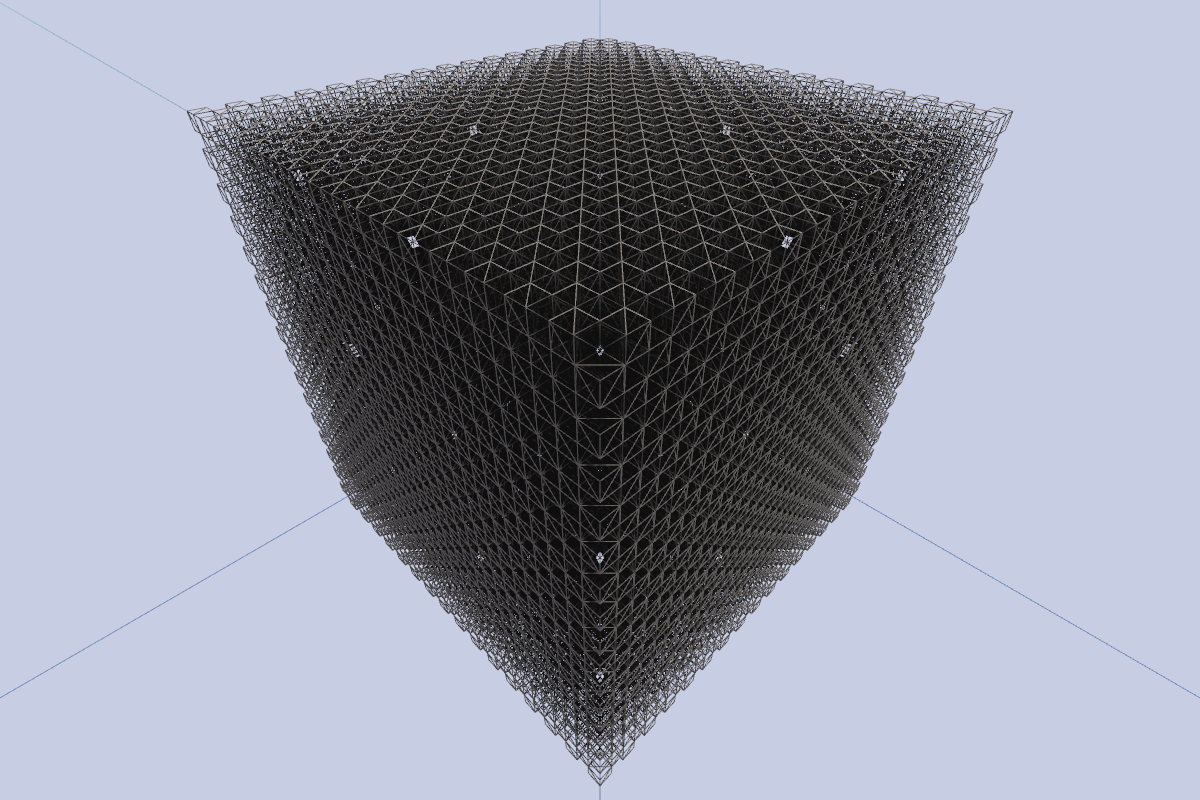
\includegraphics[width=.7\textwidth]{fps-cube.png}};
		\spy on (-3.8,2.65) in node [right] at (-10,2);
		\spy on (0.25,.65) in node [right] at (-10,-2);
	\end{tikzpicture} 
	\caption{Halbwürfel Bild}\label{fig:cube}
\end{figure}
Da die Anzahl der zu zeichnenden Objekte in dem ersten Szenario relativ gering ist, wird diese in Szenario 2, das in Abbildung~\ref{fig:cube} veranschaulicht ist, erhöht. In diesem Szenario wird ein Bereich von $32 \times 32 \times 32$ Blöcken so befüllt, dass an jeder zweiten Stelle ein Block ist. Zweidimensional entspricht das einem Schachbrettmuster. Die Anzahl der platzierten Blöcke ist damit $\frac{1}{2}\cdot32^3 = 16384$. Die Anzahl der zu zeichnenden Dreiecke ist $16384\cdot6 + 5= = 98309$.

Aufgrund der Anordnung wären allerdings nur wenige Blöcke sichtbar. Daher wird das Drahtgittermodell gezeichnet, also nur die Kanten der zu zeichnenden Dreiecke. Dennoch kann hier nicht mehr sichergestellt werden, dass auch tatsächlich alle Elemente gezeichnet werden, da selbst mit dem Drahtgittermodell an vielen Stellen Polygone überdeckt werden. Durch die Darstellung als Drahtgittermodell lassen sich nun auch die Kanten der Skybox erkennen und man sieht, dass das Dreiecke in der oberen rechten Ecke nicht gezeichnet wird. 

\begin{figure}[!htb]
	\fpsplot{seed-0-cube}
	\caption{Seed 0 Halb-Würfel}\label{fig:seed-0-cube-fps}
\end{figure}
Der Verlauf der Framerate für Szenario 2 ist in Abbildung~\ref{fig:seed-0-cube-fps} dargestellt. In SystemA werden Frames ab Sekunde $11$ erzeugt, in SystemB ab Sekunde $13$. Die mittlere Framerate in SystemA ist \SI{238}{\fps} und in SystemB \SI{394}{\fps}. Damit erhöht sich die Framerate in SystemB um \SI{66}{\percent}. Dieser Wert ist deutlich geringer als in Szenario 1. Die Frameraten bleiben in beiden Systemen sehr konstant.

\begin{figure}[!htb]
	\cpuplot{seed-0-cube}
	\caption{Seed 0 Halb-Würfel}\label{fig:seed-0-cube-cpu}
\end{figure}
Die Auslastung der CPU in Szenario 2, zu sehen in Abbildung~\ref{fig:seed-0-cube-cpu}, gestaltet sich vergleichbar zu der in Szenario 1. Die Mittelwerte sind mit \SI{14}{\percent} in SystemA und \SI{19}{\percent} in SystemB nach Rundung identisch zu Szenario 1.
Auffällig ist, dass SystemB wie in Szenario 1 in den ersten Sekunden, während des Starts der Blocklib, zwei Auslastungsspitzen besitzt (\SI{32}{\percent} und \SI{50}{\percent}). SystemA dagegen besitzt nur eine (\SI{46}{\percent}). Eine mögliche Erklärung dafür ist die Trennung von Simulation und Rendering in verschiedene Threads. Dadurch könnte es passieren, die CPU zeitweise dadurch entlastet ist, dass die GPU Zeit benötigt, um übergebene Anweisungen auszuführen, beispielsweise wenn Texturen zum Start auf die Grafikkarte geladen werden.

\begin{figure}[!htb]
	\gpuplot{seed-0-cube}
	\caption{Seed 0 Halb-Würfel}\label{fig:seed-0-cube-gpu}
\end{figure}
Die Auslastung des Halb-Würfel Szenario unterscheidet sich im Gegensatz zur CPU-Auslastung sehr von der im Hexagon-Szenario gemessenen. In Abbildung~\ref{fig:seed-0-cube-gpu} ist die gemessene GPU-Auslastung zeitlich aufgetragen. Anders als in Szenario 1 ist in beiden Systemen der Unterschied in der Auslastung unübersehbar. SystemB nutzt nach dem Start nahezu \SI{100}{\percent} der Leistung der GPU, während SystemA nur etwa \SI{60}{\percent} Auslastung erzeugt. Durchschnittlich liegt SystemB damit bei \SI{70}{\percent} Auslastung über die gesamte Messdauer und SystemA bei \SI{45}{\percent}. Betrachtet man nur die Auslastung nach dem Start lässt sich eine Steigerung der Auslastung um $\frac{100}{60}\si{\percent} \approx 67\si{\percent}$ errechnen. Das entspricht der Steigerung der \si{\fps}. In den weiteren Szenarien wird sich zeigen, ob das nur Zufall ist oder auf ein Muster schließen lässt.

\begin{figure}[!htb]
	\memplot{seed-0-cube-single-mem.csv}
	\memplot{seed-0-cube-multi-mem.csv}
	\caption{Seed 0 Halb-Würfel}\label{fig:seed-0-cube-mem}
\end{figure} 
Die Speichernutzung in Szenario 2 wird in Abbildung~\ref{fig:seed-0-cube-mem} gezeigt. Der Speicherverbrauch von SystemA unterscheidet sich im Vergleich zum Hexagon-Szenario kaum